\documentclass[12pt,a4paper]{article}
\usepackage[utf8]{inputenc}
\usepackage[spanish]{babel}
\usepackage{amsmath, amssymb}
\usepackage{graphicx}
\usepackage{booktabs}
\usepackage{geometry}
\usepackage[hidelinks]{hyperref}
\usepackage{enumitem}
\usepackage{fancyhdr}
\usepackage{float}
\usepackage{caption}
\usepackage{siunitx}
\usepackage{titlesec}
\usepackage{authblk}

\geometry{margin=2.5cm}

\pagestyle{fancy}
\fancyhf{}
\rhead{Modelo SEIR con vacunación}
\lhead{Informe Científico}
\rfoot{\thepage}
\setlength{\headheight}{14.5pt} % Fix for fancyhdr warning

\titleformat{\section}{\normalfont\Large\bfseries}{\thesection}{1em}{}
\titleformat{\subsection}{\normalfont\large\bfseries}{\thesubsection}{1em}{}

\title{\textbf{Modelado Matemático de la Transmisión de Leptospirosis con Estrategias de Vacunación Basadas en Dinámicas Estacionales e Infecciosas}}
\author{Richard Alejandro Matos Arderí}
\newcommand{\tutor}{José Carlos}
\newcommand{\institucion}{Instituto Finlay de Vacunas}
\newcommand{\universidad}{Facultad de Matemática y Computación, Universidad de La Habana}
\newcommand{\grado}{Tercer año de Licenciatura en Ciencia de la Computación}
\newcommand{\correo}{\texttt{matosrichard58@gmail.com}}

\date{
    \begin{tabular}{rl}
        \textbf{Grado:} & \grado \\
        \textbf{Universidad:} & \universidad \\
        \textbf{Correo:} & \correo \\
        \textbf{Institución:} & \institucion \\
         \textbf{Tutor:} & \tutor \\
         \textbf{Correo del tutor:} & \texttt{jose.carlos@institutofinlay.cu}   
    \end{tabular}
    \\[1em]
    \today
}
\date{Mayo de 2025}

\begin{document}

\maketitle
\thispagestyle{empty}
\newpage

\tableofcontents
\newpage

% ================================
\section{Introducción}
La leptospirosis es una enfermedad infecciosa bacteriana zoonósica causada por la bacteria \textit{Leptospira interrogans}. Se transmite principalmente por contacto con orina de roedores infectados o ambientes contaminados. Su prevalencia es mayor en regiones tropicales y en zonas urbanas marginales con alta presencia de ratas.

Este estudio propone un modelo matemático compartimental para analizar la transmisión de la leptospirosis y evaluar el impacto de estrategias de vacunación. Se exploran escenarios con y sin intervención vacunal y se evalúa la relación costo-beneficio de aplicar un programa de vacunación.

El informe está organizado como sigue: se formula el modelo matemático base (SEIR), se presenta su extensión con vacunación, se reportan los resultados de simulación y se discuten los análisis de sensibilidad y costo-beneficio.

\newpage

% ================================
\section{Formulación del Modelo SEIR Básico}

\subsection{Supuestos y condiciones iniciales}
\begin{itemize}
\item La población humana total, denotada como $N_{0,h}$, se divide en susceptibles ($S_h$), expuestos ($E_h$), infectados ($I_h$) y recuperados ($R_h$).
\item La transmisión ocurre por contacto con roedores infectados o ambientes contaminados.
\item La población de roedores incluye susceptibles ($S_v$), infectados ($I_v$) y recuperados ($R_v$).
\item Existe una población ambiental de bacterias patógenas $B_l$.
\end{itemize}

\subsection{Compartimentos y diagrama}
\begin{center}
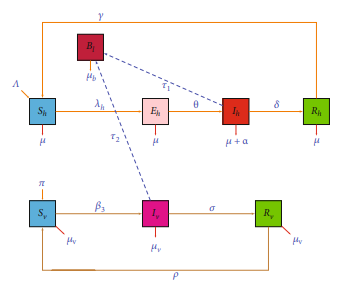
\includegraphics[width=0.9\textwidth]{Images/modelo_seir.png}
\captionsetup{hypcap=false}
\captionof{figure}{Diagrama de flujos del modelo SEIR con roedores y ambiente.}
\end{center}

\subsection{Ecuaciones diferenciales}

El sistema completo de ecuaciones diferenciales es:
% Humanos
\begin{align*}
\frac{dS_h}{dt} &= \Lambda + \gamma R_h - \lambda_h S_h - \mu S_h \\
\frac{dE_h}{dt} &= \lambda_h S_h - (\theta + \mu) E_h \\
\frac{dI_h}{dt} &= \theta E_h - (\alpha + \delta + \mu) I_h \\
\frac{dR_h}{dt} &= \delta I_h - (\gamma + \mu) R_h
\end{align*}

% Vectores (roedores)
\begin{align*}
\frac{dS_v}{dt} &= \Pi + \rho R_v - (\beta_3(t) I_h + \mu_v) S_v \\
\frac{dI_v}{dt} &= \beta_3(t) I_h S_v - (\sigma + \mu_v) I_v \\
\frac{dR_v}{dt} &= \sigma I_v - (\rho + \mu_v) R_v
\end{align*}

% Ambiente
\begin{align*}
\frac{dB_l}{dt} &= \tau_1 I_h + \tau_2 I_v - \mu_b B_l
\end{align*}

\textbf{Donde:}
\begin{itemize}
    \item $S_h, E_h, I_h, R_h$: humanos susceptibles, expuestos, infectados y recuperados.
    \item $S_v, I_v, R_v$: roedores susceptibles, infectados y recuperados.
    \item $B_l$: bacterias patógenas en el ambiente.
    \item $\lambda_h$: fuerza de infección humana, dependiente del tiempo y del ambiente.

    En el modelo, la fuerza de infección humana se define como:
    \[
    \lambda_h = \frac{\beta_2(t) B_l}{\kappa + B_l} + \beta_1(t) I_v
    \]
    donde $\lambda_h$ representa la tasa instantánea a la que los susceptibles humanos se infectan, considerando tanto la transmisión ambiental como la proveniente de roedores infectados. Nótese que $\beta_1(t)$ y $\beta_2(t)$ son funciones estacionales (ver más abajo).
\end{itemize}

\subsection{Parámetros y criterios poblacionales}
\begin{table}[H]
\centering
\begin{tabular}{@{}lllll@{}}
\toprule
\textbf{Parámetro} & \textbf{Descripción} & \textbf{Valor} & \textbf{Unidades} & \textbf{Fuente} \\
\midrule
$\Lambda$ & Tasa de reclutamiento  
           & $\mu \times N_{0,h}$ & humano/día & \cite{paisanwarakiat2021} \\
          & humana &  &  &  \\
$\Pi$ & Tasa de reclutamiento  
      & 2 & roedor/día & \cite{paisanwarakiat2021} \\
      & de roedores  &  &  &  \\
$\beta_{1,m}$ & Transmisión roedor- 
              & 0.00033 & 1/(roedor·día) & \cite{engida2022} \\
              & humano (promedio) &  &  &  \\
$\beta_{2,m}$ & Transmisión ambiente-
              & 0.0815 & 1/día & \cite{engida2022} \\
              & humano (promedio)  &  &  &  \\
$\beta_{3,m}$ & Transmisión humano-
              & 0.0007 & 1/(humano·día) & \cite{engida2022} \\
              & roedor (promedio)  &  &  &  \\
$\gamma$ & Pérdida de  
         & 0.089 & 1/día & \cite{khan2014} \\
         & inmunidad humana &  &  &  \\
$\mu$ & Mortalidad natural 
      & 0.0009 & 1/día & \cite{alemneh2020,paisanwarakiat2021} \\
      & humana  &  &  &  \\
$\mu_v$ & Mortalidad natural 
        & 0.0029 & 1/día & \cite{alemneh2020} \\
        & roedores  &  &  &  \\
$\mu_b$ & Mortalidad bacterias 
        & 0.05 & 1/día & \cite{minter2019} \\
        &  &  &  &  \\
$\theta$ & Progresión expuesto
         & 0.092 & 1/día & \cite{khan2012} \\
         &  a infectado  &  &  &  \\
$\alpha$ & Mortalidad por 
         & 0.04 & 1/día & \cite{engida2022} \\
         & enfermedad  &  &  &  \\
$\delta$ & Recuperación humana 
         & 0.072 & 1/día & \cite{engida2022} \\
         &  &  &  &  \\
$\rho$ & Pérdida de inmunidad
       & 0.083 & 1/día & \cite{engida2022} \\
       &  roedores  &  &  &  \\
$\sigma$ & Recuperación roedores 
         & 0.064 & 1/día & \cite{engida2022} \\
         &  &  &  &  \\
$\kappa$ & Constante de saturación
         & 10000 & - & \cite{engida2022} \\
         &  ambiental  &  &  &  \\
$\tau_1$ & Liberación de patógeno 
         & 0.06 & bacterias/(humano·día) & \cite{minter2019} \\
         &  por humanos &  &  &  \\
$\tau_2$ & Liberación de patógeno 
         & 0.2 & bacterias/(roedor·día) & \cite{minter2019} \\
         & por roedores  &  &  &  \\
\bottomrule
\end{tabular}
\caption{Parámetros del modelo SEIR extendido con roedores y ambiente. Los valores de $\beta_1$, $\beta_2$ y $\beta_3$ corresponden a los promedios anuales y se usan como base para las funciones estacionales.}
\end{table}



\subsection{Parámetros estacionales o dependientes del tiempo}
Las tasas de transmisión $\beta_1$, $\beta_2$ y $\beta_3$ varían estacionalmente según:

\begin{align*}
\beta_i(t) = \beta_{i,m} \left[1 + A \cos\left(2\pi \frac{m(t) - t_{\text{pico}}}{12}\right)\right]
\end{align*}

donde:
\begin{itemize}
    \item $\beta_{i,m}$: valor promedio anual de la tasa de transmisión ($i=1,2,3$).
    \item $A$: amplitud estacional ($0 < A < 1$). Valores cercanos a 0 indican poca variación estacional en la transmisión, mientras que valores altos (próximos a 1) reflejan una marcada estacionalidad. Un valor medio (por ejemplo, $A=0.4$) implica una variación moderada en la tasa de transmisión a lo largo del año.
    \item $m(t)$: mes correspondiente al día $t$ ($m(t) = \lfloor t/30 \rfloor \bmod 12 + 1$).
    \item $t_{\text{pico}}$: mes de máximo estacional.
\end{itemize}

Por ejemplo, para la transmisión ambiente-humano:
\[\
\beta_2(t) = \beta_{2,0} \left[1 + 0.4 \cos\left(2\pi \frac{m(t) - 2}{12}\right)\right]
\]

Este mismo esquema se aplica a $\beta_1$ y $\beta_3$.

\newpage

% ================================
\section{Extensión del Modelo con Vacunación}

\subsection{Modificación del sistema y nuevas ecuaciones}

Para modelar la intervención vacunal, se añade el compartimento $V_h$ (humanos vacunados) y se modifica la dinámica de los susceptibles humanos. La adición del compartimento $V_h$ (humanos vacunados) se justifica principalmente porque la inmunidad temporal adquirida tras la recuperación de la enfermedad no es necesariamente igual a la inmunidad conferida por la vacuna. Esta distinción permite modelar de manera más realista el comportamiento de la población, ya que la duración y eficacia de la inmunidad pueden diferir entre ambos grupos. Además, resulta de especial interés analizar la evolución del compartimento $V_h$ para evaluar el impacto de la vacunación en la dinámica de la enfermedad y en la protección de la población a lo largo del tiempo. Además, la tasa de vacunación diaria $\phi$ se modela como una función dinámica $\nu(t)$ que depende de la situación epidemiológica y la estacionalidad.

Las ecuaciones modificadas y añadidas son:

\begin{align*}
\frac{dS_h}{dt} &= \Lambda + \gamma R_h + \omega V_h - \lambda_h S_h - \mu S_h - \nu(t) \varepsilon S_h \\
\frac{dV_h}{dt} &= \nu(t) \varepsilon S_h - (\omega + \mu) V_h
\end{align*}

El resto de ecuaciones para roedores y ambiente permanecen igual que en el modelo base.

\textbf{Donde:}
\begin{itemize}
    \item $V_h$: humanos vacunados.
    \item $\nu(t)$: tasa diaria de vacunación dinámica, definida abajo.
    \item $\varepsilon$: eficacia de la vacuna.
    \item $\omega$: tasa de pérdida de inmunidad vacunal.
    \item El resto de variables y parámetros se mantienen como antes.
\end{itemize}

\subsection{Definición de la tasa de vacunación dinámica}

La tasa diaria de vacunación $\nu(t)$ se formula como:

\[
\nu(t) = \nu_{\max} \cdot \left( \frac{I_h(t)}{I_h(t) + K} \right) \cdot \left( \frac{\overline{\beta}(m(t))}{\beta_{\max}} \right)
\]

donde:
\begin{itemize}
    \item $\nu_{\max}$: tasa máxima alcanzable de vacunación diaria (por ejemplo, 1\% de susceptibles por día).
    \item $I_h(t)$: número de humanos infectados en el tiempo $t$.
    \item $K$: constante de saturación (1\% de la población humana inicial).
    \item $\overline{\beta}(m(t))$: promedio mensual de las tasas de transmisión ambiente-humano, roedor-humano y humano-roedor para el mes correspondiente, es decir,
    \[
    \overline{\beta}(m) = \frac{\overline{\beta}_1(m) + \overline{\beta}_2(m) + \overline{\beta}_3(m)}{3}
    \]
    \item $\beta_{\max}$: valor promedio de los máximos anuales de las tres tasas, es decir,
    \[
    \beta_{\max} = \frac{1}{3} \left( \max_m \overline{\beta}_1(m) + \max_m \overline{\beta}_2(m) + \max_m \overline{\beta}_3(m) \right)
    \]

    \item $m(t)$: mes correspondiente al día $t$.
\end{itemize}

\textbf{Justificación:} Esta función refleja una política de vacunación reactiva y estratégica, aumentando la vacunación cuando hay más infectados y cuando la transmisión estacional es alta. Así, se evita sobrevacunar en periodos de bajo riesgo y se prioriza la intervención en brotes y épocas críticas.

\subsection{Parámetros añadidos y dependientes del tiempo}

\begin{table}[H]
\centering
\begin{tabular}{@{}lllll@{}}
\toprule
\textbf{Parámetro} & \textbf{Descripción} & \textbf{Valor} & \textbf{Unidades} & \textbf{Fuente} \\
\midrule
$\phi$ ($\nu_{\max}$) & Tasa máxima de vacunación diaria & 0.01 & 1/día & Supuesto \\
$\varepsilon$ & Eficacia de la vacuna & 0.78 & - & Supuesto \\
$\omega$ & Pérdida de inmunidad vacunal & $1/180$ & 1/día & Supuesto \\
\bottomrule
\end{tabular}
\caption{Parámetros adicionales y dependientes del tiempo para la vacunación.}
\end{table}

Las tasas de transmisión $\beta_1$, $\beta_2$ y $\beta_3$ siguen variando estacionalmente como en el modelo base:


\subsection{Argumentación de las modificaciones}

Las modificaciones introducidas buscan reflejar la realidad de las campañas de vacunación, que suelen intensificarse ante brotes o en periodos de mayor riesgo estacional. El uso de una tasa dinámica $\nu(t)$ permite modelar respuestas adaptativas del sistema de salud, optimizando recursos y maximizando el impacto preventivo de la vacunación. Además, la inclusión de la pérdida de inmunidad vacunal ($\omega$) y la eficacia real de la vacuna ($\varepsilon$) permite evaluar escenarios más realistas y comparables con datos empíricos.

\subsection{Datos de la vacuna Vax-SPIRAL}

La vacuna considerada en este modelo es \textbf{Vax-SPIRAL}, desarrollada para la prevención de leptospirosis. Los parámetros usados son:

\begin{itemize}
    \item \textbf{Eficacia vacunal} ($\varepsilon = 0.78$): Basado en estudios clínicos y reportes de efectividad de Vax-SPIRAL en poblaciones expuestas, donde se ha observado una reducción del 78\% en la incidencia de la enfermedad entre vacunados respecto a no vacunados.
    \item \textbf{Duración de la inmunidad vacunal} ($\omega = 1/180$): Se asume una duración promedio de 6 meses para la inmunidad conferida por la vacuna, acorde a la literatura y recomendaciones del fabricante, lo que implica una tasa de pérdida de inmunidad de $1/180$ por día.
    \item \textbf{Tasa máxima de vacunación} ($\nu_{\max} = 0.01$): Se considera que, logísticamente, es posible vacunar hasta el 1\% de la población susceptible por día en campañas intensivas, valor ajustable según la capacidad del sistema de salud.
\end{itemize}

\newpage

% ================================
\section{Resultados del Modelo}

\subsection{Escenarios simulados y parámetros para el sur de Brasil}

Para ilustrar el comportamiento del modelo, se simulan dos escenarios principales:
\begin{enumerate}
    \item \textbf{Escenario 1: Sin vacunación} (estrategia base, $\nu(t) = 0$).
    \item \textbf{Escenario 2: Con vacunación dinámica} (estrategia reactiva, $\nu(t)$ según la función propuesta).
\end{enumerate}

\textbf{Nota sobre la interpretación y el alcance temporal de los resultados:} Los resultados que se presentan y analizan a continuación corresponden a simulaciones realizadas durante un periodo de un año, lo que permite visualizar de manera clara la dinámica estacional y el impacto de las estrategias de vacunación en un ciclo anual típico. Sin embargo, el software desarrollado y anexado al final de este informe permite al usuario seleccionar el horizonte temporal de la simulación según sus necesidades, facilitando así el análisis de escenarios a corto, mediano o largo plazo de manera interactiva y personalizada.

\textbf{Justificación de parámetros para el sur de Brasil:}
\begin{itemize}

    \item \textbf{Amplitud estacional $A=0.4$}: En el sur de Brasil, la leptospirosis muestra marcada estacionalidad, con picos en la temporada de lluvias y calor. Un valor de $A=0.4$ representa una variación moderada a alta en la transmisión a lo largo del año, acorde a reportes epidemiológicos regionales.
    \item \textbf{Mes pico $t_{\textit{pico}}=2$ (febrero)}: Los brotes suelen alcanzar su máximo en febrero, coincidiendo con el final del verano austral y el periodo de mayor precipitación.
    \item \textbf{Poblaciones iniciales:}
    \begin{itemize}
        \item Humanos susceptibles $S_h(0) = 270$
        \item Humanos expuestos $E_h(0) = 20$
        \item Humanos infectados $I_h(0) = 10$
        \item Humanos recuperados $R_h(0) = 0$
        \item Roedores susceptibles $S_v(0) = 510$
        \item Roedores infectados $I_v(0) = 10$
        \item Roedores recuperados $R_v(0) = 0$
        \item Bacterias ambientales $B_l(0) = 100$
        \item Humanos vacunados $V_h(0) = 0$
    \end{itemize}
    Estos valores reflejan una población humana y de roedores de tamaño moderado, con un brote inicial activo y un ambiente contaminado, representativo de una ciudad mediana del sur de Brasil.
\end{itemize}

\subsection{Simulación: comparación conjunta}

\subsubsection{Análisis de la Dinámica de Infectados (\texorpdfstring{$I_h$}{Ih})}


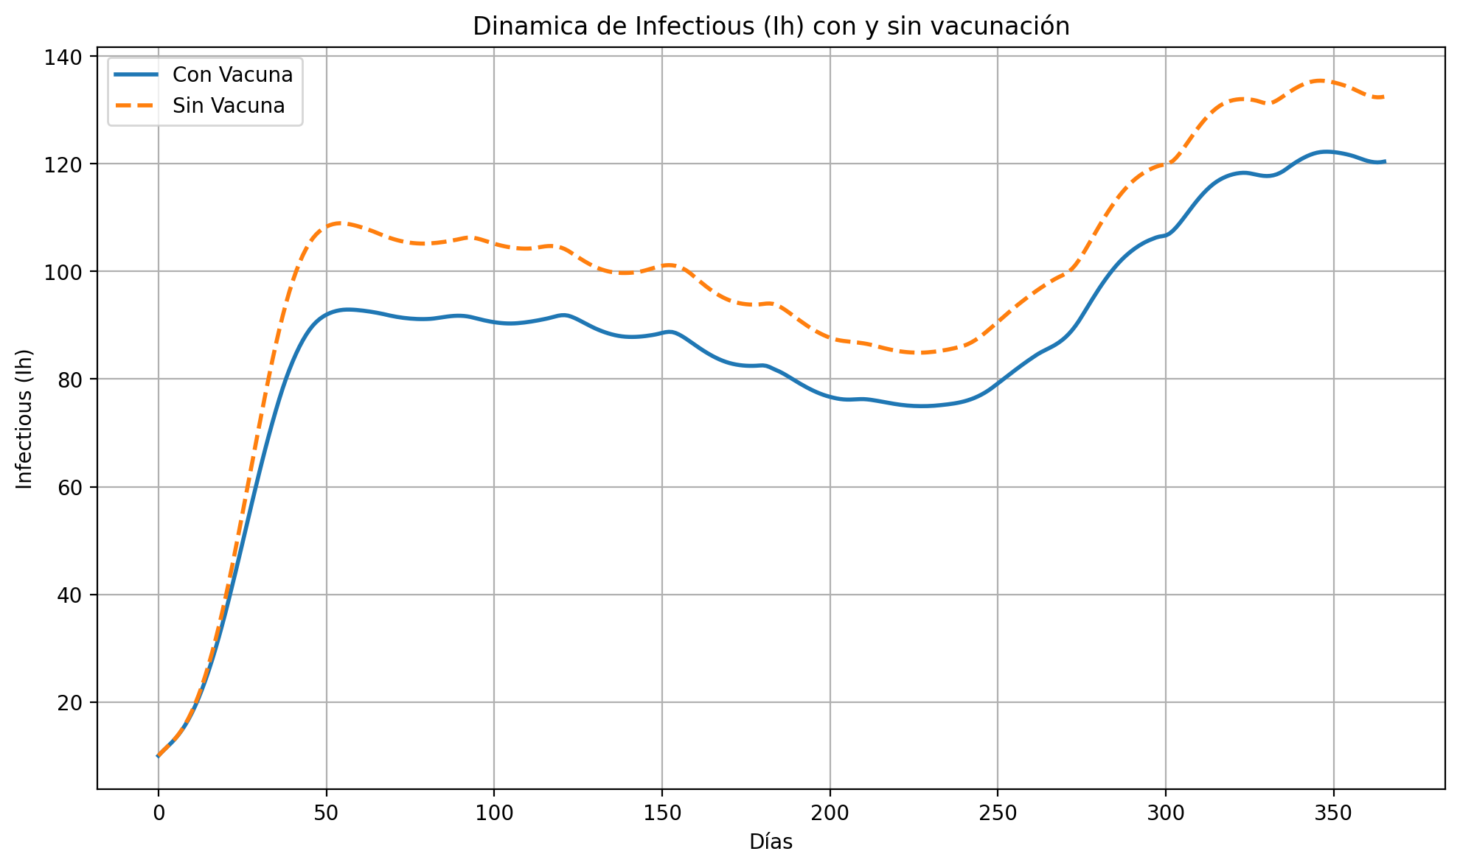
\includegraphics[width=0.85\textwidth]{Images/infectados.png}
\captionof{figure}{Evolución de infectados: comparación entre escenarios sin vacunación y con vacunación dinámica.}

La Figura  muestra la evolución de la población de individuos infectados humanos ($I_h$) durante un año bajo dos escenarios: con vacunación adaptativa (línea azul continua) y sin vacunación (línea naranja discontinua). En ambos casos, la tasa de transmisión presenta estacionalidad, con picos en los meses lluviosos (principalmente febrero), lo que es consistente con estudios epidemiológicos recientes en regiones endémicas \cite{pijnacker2019}.

\paragraph{Fase inicial (días 0–60).} Ambas curvas presentan un ascenso rápido, coincidiendo con el inicio de la temporada de alta transmisión. Sin embargo, el escenario sin vacunación alcanza un valor máximo de más de 110 infectados alrededor del día 50, mientras que el escenario con vacunación se estabiliza antes, en torno a 90 casos.

\paragraph{Fase intermedia (días 60–200).} Se observa un efecto de control en la curva con vacunación, donde los niveles de $I_h$ se mantienen más bajos y estables que en el escenario sin intervención. Esto refleja el impacto de la estrategia vacunal reactiva, que se activa en función del número de infectados y la intensidad de la transmisión.

\paragraph{Fase tardía (días 200–360).} A partir del día 250 ocurre un segundo repunte epidémico más marcado en el escenario sin vacunación, alcanzando máximos de hasta 135 infectados. Este comportamiento podría estar asociado a la pérdida de inmunidad en individuos recuperados y a la estacionalidad secundaria, tal como se ha reportado en regiones tropicales donde se observan múltiples oleadas anuales de leptospirosis.

\paragraph{Comparación y eficacia.} En todo el intervalo, el número de infectados es consistentemente menor en el escenario con vacunación, con una diferencia acumulada significativa en el área bajo la curva. Esto demuestra que la intervención vacunal dinámica no solo atenúa los picos de infección, sino que reduce de forma sostenida la carga de enfermedad.

\paragraph{Conclusión.} La vacunación adaptativa modulada por indicadores epidemiológicos permite mitigar eficazmente la incidencia de leptospirosis, especialmente en entornos con fuerte estacionalidad. Esto coincide con evidencia científica sobre la utilidad de intervenciones preventivas focalizadas durante los periodos de mayor riesgo \cite{pijnacker2019}.




\subsubsection{Análisis de la Dinámica de los Susceptibles (\texorpdfstring{$S_h$}{Sh})}

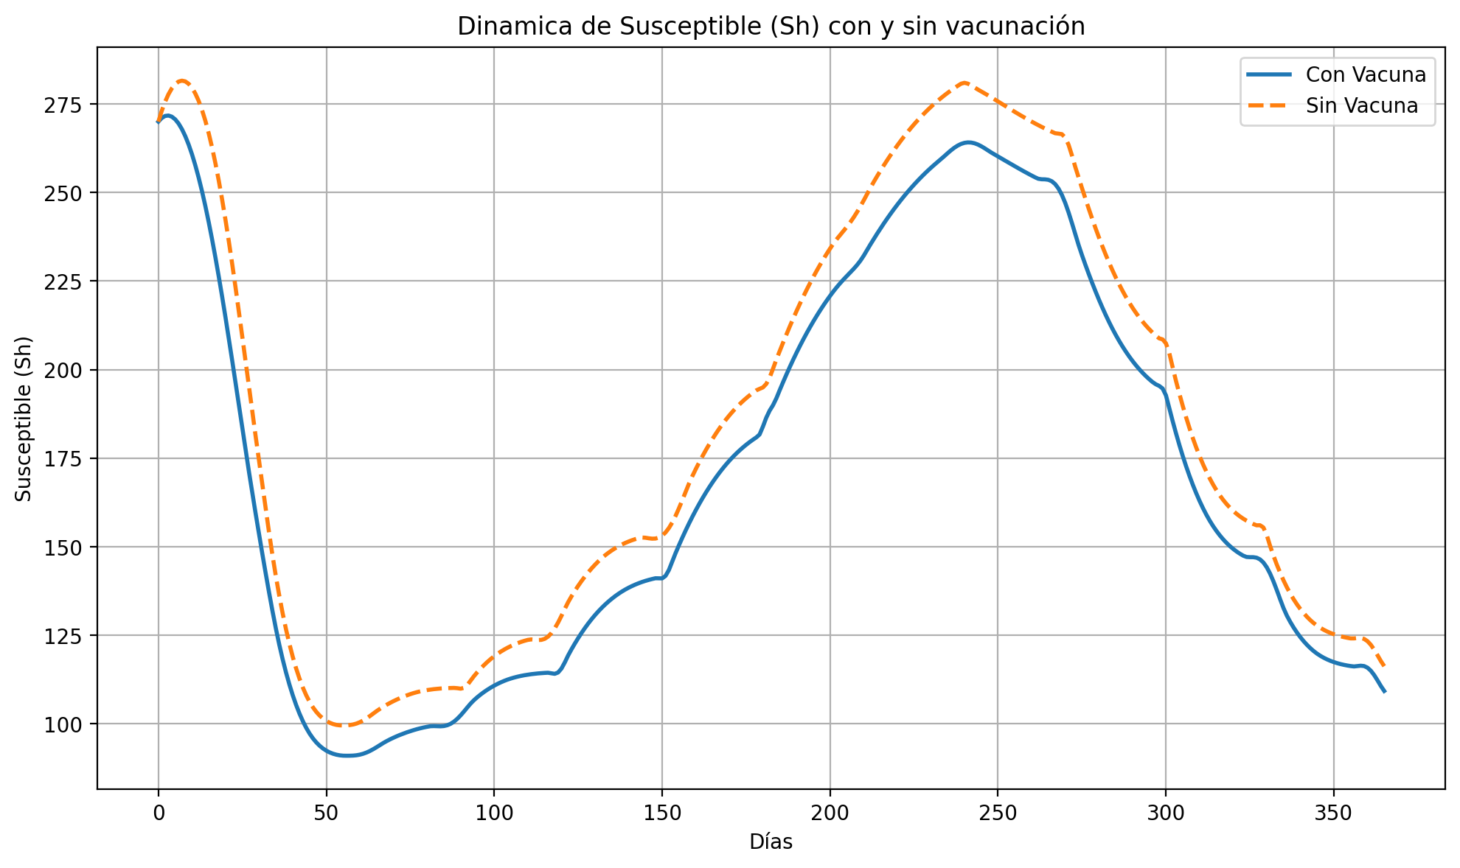
\includegraphics[width=0.85\textwidth]{Images/susceptibles.png}
\captionof{figure}{Evolución de susceptibles: comparación entre escenarios sin y con vacunación.}

Se muestra la evolución de la población susceptible humana a lo largo de un año bajo dos escenarios: con vacunación (línea azul continua) y sin vacunación (línea naranja discontinua). 


\paragraph{Tendencia general.} Ambas curvas presentan una evolución cíclica, lo cual es típico de modelos epidemiológicos con transmisión estacional. Se observa un descenso abrupto inicial, una fase de recuperación intermedia y un segundo descenso hacia mediados del año.

\paragraph{Fase inicial (días 0--60).} La población susceptible cae rápidamente en ambos escenarios debido a la alta tasa de transmisión en febrero. Sin embargo, la curva sin vacunación muestra una caída más pronunciada, indicando una mayor propagación del contagio. En el escenario con vacunación, el efecto inmunizante reactivo modula la velocidad de pérdida de susceptibles.

\paragraph{Fase de estabilización (días 60--200).} Tras el primer brote, ambas curvas muestran una recuperación gradual del número de susceptibles. En el escenario con vacunación, dicha recuperación es más rápida debido a la menor tasa de infección y la reincorporación de personas desde los compartimentos $R_h$ y $V_h$ por pérdida de inmunidad.

\paragraph{Segundo brote (días 200--300).} Se observa una segunda disminución en ambas curvas, presumiblemente asociada a una estacionalidad secundaria o a la acumulación de individuos susceptibles. Nuevamente, la curva sin vacunación desciende más abruptamente, mientras que el modelo con vacuna muestra una caída más moderada y una recuperación anticipada.

\paragraph{Interpretación general.} La estrategia vacunal reactiva permite suavizar las oscilaciones de la población susceptible, reduciendo la magnitud y duración de los brotes. Aunque no evita completamente las infecciones, disminuye su impacto. Esto valida la utilidad de políticas de vacunación ajustadas dinámicamente a indicadores epidemiológicos y estacionales.

\paragraph{Recomendaciones.} Se recomienda implementar campañas vacunales intensivas previas al mes de febrero, monitorear la pérdida de inmunidad e integrar medidas ambientales para reforzar el efecto protector observado.

\subsubsection{Análisis de la Dinámica de Expuestos (\texorpdfstring{$E_h$}{Eh})}

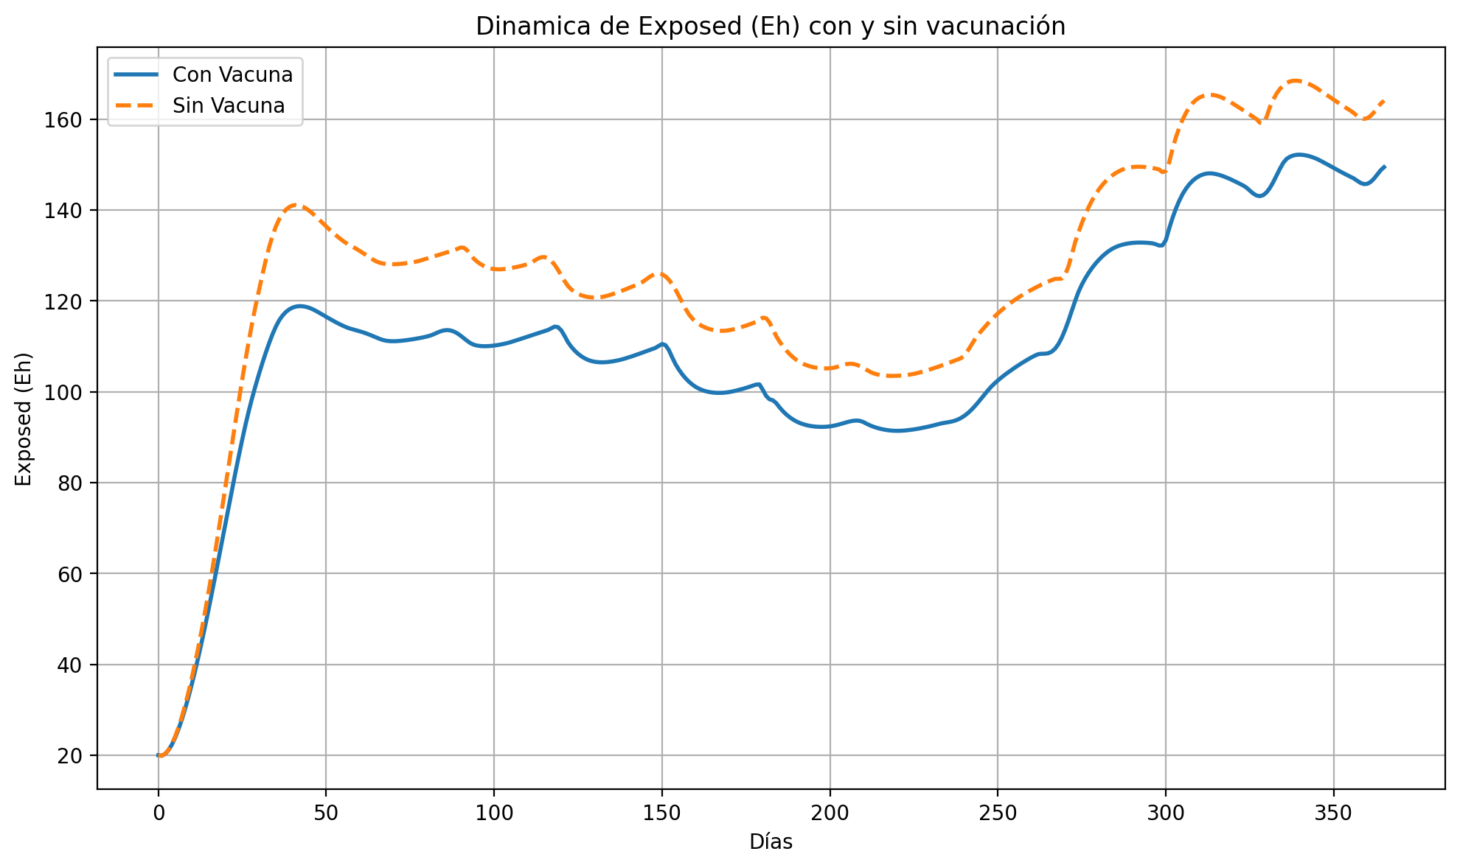
\includegraphics[width=0.85\textwidth]{Images/expuestos.png}
\captionof{figure}{Evolución de expuestos: comparación entre escenarios sin y con vacunación.}


La Figura muestra la evolución del número de individuos expuestos ($E_h$), es decir, aquellos que han sido infectados por leptospiras pero aún no presentan síntomas ni son infecciosos. Se comparan los escenarios con vacunación adaptativa (línea azul continua) y sin vacunación (línea naranja discontinua), durante un año.


\paragraph{Interpretación general.} La población expuesta sigue una evolución similar a la de los infectados, aunque desfasada debido al periodo de incubación de la leptospirosis, que suele oscilar entre 5 y 14 días, con un promedio de 10 días según el CDC \cite{cdc2024}. Este compartimento refleja el impacto temprano de la transmisión, antes de que los casos se manifiesten clínicamente.

\paragraph{Primer ascenso (días 0–50).} Ambos escenarios presentan un rápido incremento de individuos expuestos durante los primeros 50 días, coincidiendo con la temporada de mayor transmisión. El escenario sin vacunación alcanza un pico superior (alrededor de 140 individuos), mientras que con vacunación este valor es moderado (~120). Esto sugiere que la vacunación reduce el ritmo de nuevas exposiciones al disminuir la circulación del patógeno en el ambiente.

\paragraph{Meseta y oscilaciones (días 60–200).} Se observa una fase de estabilización con oscilaciones suaves en ambos escenarios. El número de expuestos es sistemáticamente menor con vacunación, lo cual confirma que la estrategia vacunal está funcionando de manera preventiva en el umbral antes del desarrollo de la infección clínica.

\paragraph{Rebrote tardío (días 250–350).} Similar al compartimento $I_h$, se observa un segundo aumento de expuestos en ambos escenarios, más pronunciado sin vacunación. Esto puede explicarse por una combinación de pérdida de inmunidad, condiciones ambientales favorables al patógeno (lluvias tardías) y aumento estacional en la población de roedores.

\paragraph{Conclusión.} La vacunación no sólo reduce los casos clínicos (infectados), sino también modera la cantidad de individuos en periodo de incubación, reduciendo el potencial epidémico oculto. Esto sugiere que la vacunación tiene un efecto positivo temprano y sostenido sobre la dinámica general de la transmisión, anticipándose al desarrollo de brotes más severos.



\subsubsection{Análisis de la Dinámica de Recuperados (\texorpdfstring{$R_h$}{Rh})}

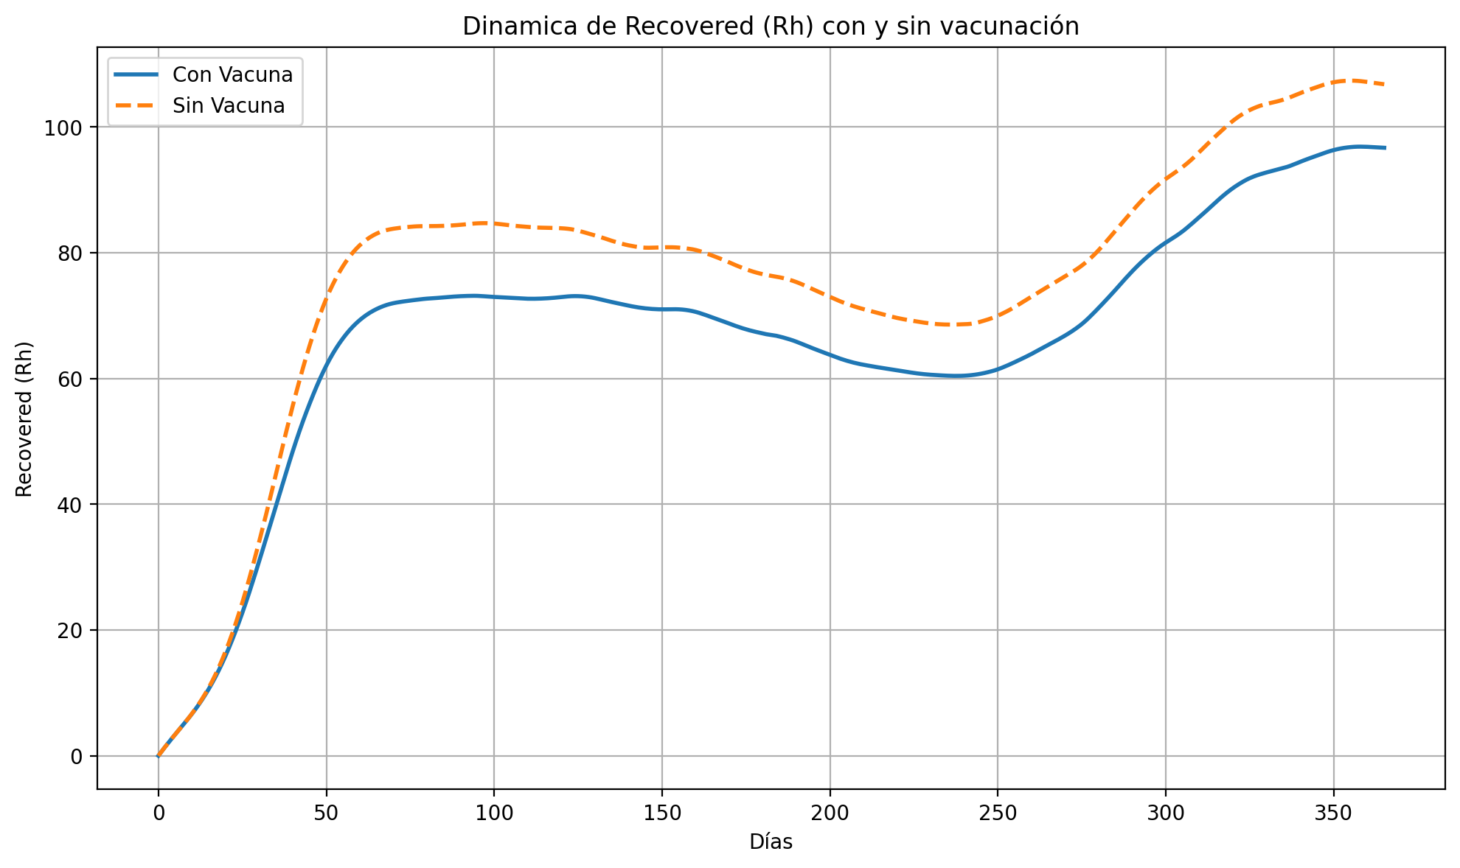
\includegraphics[width=0.85\textwidth]{Images/recuperados.png}
\captionof{figure}{Evolución de recuperados: comparación entre escenarios sin y con vacunación.}


La Figura muestra la evolución de la población humana recuperada ($R_h$) a lo largo de un año. Se comparan los escenarios con vacunación adaptativa (línea azul continua) y sin vacunación (línea naranja discontinua), en un entorno con estacionalidad en la transmisión de leptospirosis.

\paragraph{Fase inicial (días 0–80).} Ambas curvas muestran un aumento progresivo de individuos recuperados como consecuencia directa del primer brote infeccioso. La curva sin vacunación alcanza valores más altos, lo cual es esperable ya que, en ausencia de intervención, más individuos pasan por la enfermedad y eventualmente se recuperan.

\paragraph{Meseta y descenso (días 80–240).} Tras el primer pico de recuperación, ambas curvas entran en una fase de meseta. Sin embargo, se observa una leve disminución progresiva en el número de recuperados, más acentuada en el escenario con vacunación. Esto es atribuible al parámetro $\gamma$, que modela la pérdida de inmunidad natural y devuelve individuos recuperados al compartimento de susceptibles ($S_h$).

\paragraph{Repunte final (días 250–360).} Se evidencia un segundo incremento en el número de recuperados, coincidiendo con el rebrote epidémico observado previamente en las curvas de $I_h$ y $E_h$. Nuevamente, el escenario sin vacunación alcanza un nivel superior de recuperados debido a la mayor cantidad de infecciones que ocurren.

\paragraph{Comparación e implicaciones.} Aunque el modelo con vacunación presenta un número menor de recuperados, esto no implica menor efectividad, sino que refleja una menor incidencia total de la enfermedad. Es decir, menos personas enferman y, por tanto, menos personas necesitan recuperarse. La curva con vacunación también muestra una dinámica más suave y controlada, lo que sugiere una menor presión sobre los servicios de salud.

\paragraph{Apoyo bibliográfico.} Estudios como el de Adler y Moctezuma (2010) han documentado que la inmunidad post-leptospirosis no siempre es duradera ni totalmente protectora, lo que justifica la inclusión del parámetro $\gamma$ en el modelo \cite{adler2010}. La combinación de inmunidad natural transitoria y vacunación adaptativa permite mantener una dinámica epidémica más estable y controlada.



\subsubsection{Análisis de la Dinámica de Vacunados (\texorpdfstring{$V_h$}{Vh})}

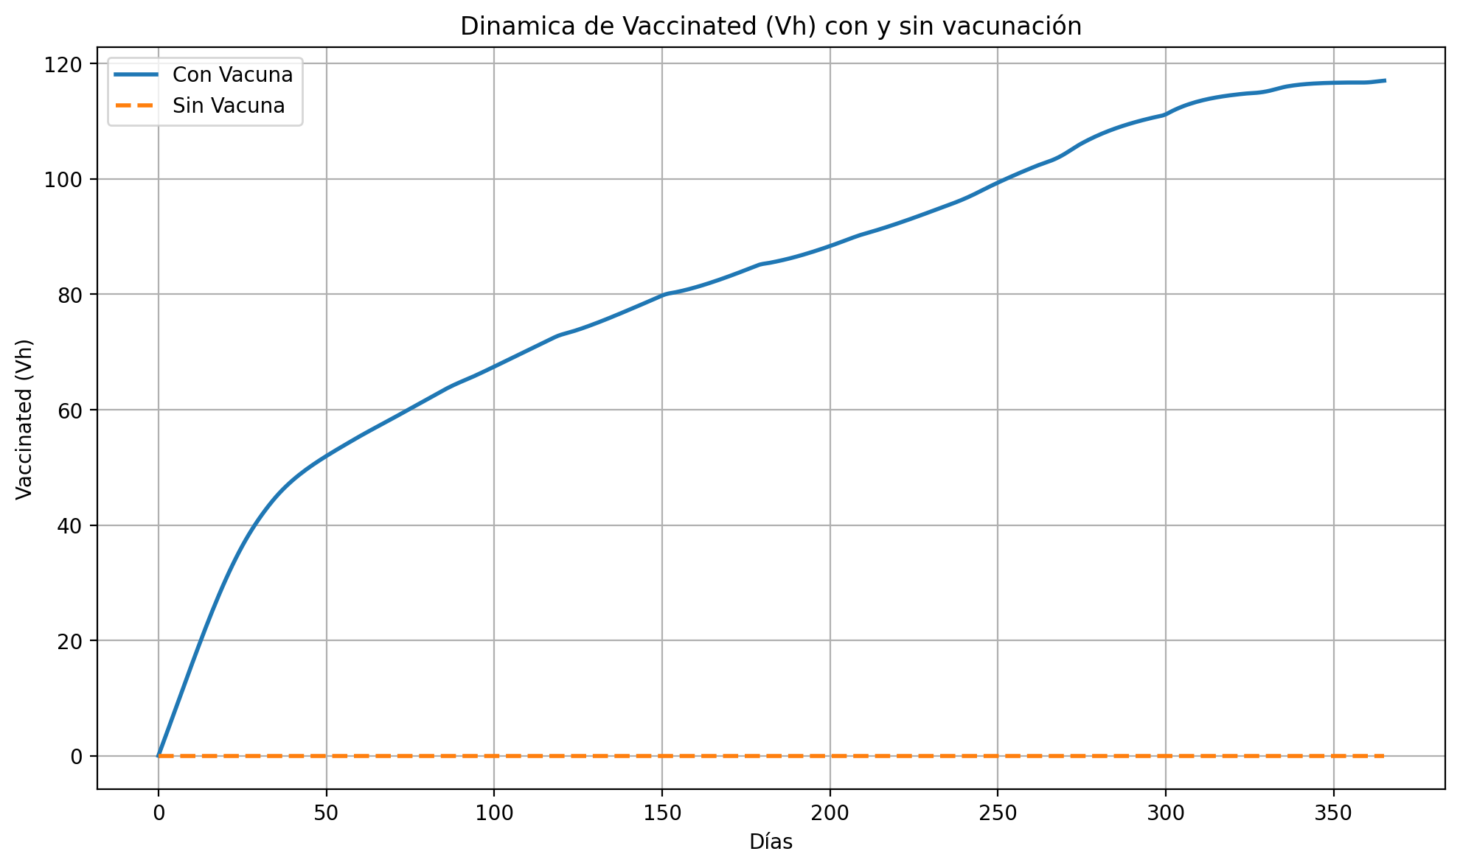
\includegraphics[width=0.85\textwidth]{Images/vacunados.png}
\captionof{figure}{Evolución de vacunados (solo escenario con vacunación).}


La Figura representa la evolución temporal del compartimento de vacunados inmunizados ($V_h$). En este compartimento se acumulan los individuos que han recibido la vacuna, esta ha sido eficaz (con probabilidad $\varepsilon$) y no han perdido aún la inmunidad inducida. Se comparan los escenarios con vacunación adaptativa (línea azul continua) y sin vacunación (línea naranja discontinua, constante en cero).

\paragraph{Crecimiento progresivo.} En el escenario con vacunación, el número de vacunados crece de forma sostenida a lo largo del año, alcanzando aproximadamente 118 individuos hacia el día 365. Esto refleja la activación continua del programa vacunal, que responde dinámicamente al aumento de $I_h(t)$ y $\beta(t)$ como parte de una estrategia adaptativa. La acumulación progresiva indica que el ritmo de vacunación ha sido suficiente para superar la tasa de pérdida de inmunidad ($\omega$).

\paragraph{Efecto protector poblacional.} La existencia de una masa crítica de individuos inmunizados reduce significativamente el riesgo de transmisión, como se observa en las curvas correspondientes a $S_h$, $E_h$ e $I_h$, donde los valores son notablemente menores bajo el escenario con vacunación. Este efecto indirecto, conocido como inmunidad de grupo parcial, es especialmente valioso en zoonosis como la leptospirosis, donde la transmisión puede ser explosiva en contextos de alta exposición ambiental.

\paragraph{Permanencia limitada.} La curva no se estabiliza completamente, lo cual indica que hay una rotación continua de personas dentro y fuera del compartimento $V_h$. Esta rotación obedece a la pérdida de inmunidad vacunal a una tasa de $1/180$ días (aproximadamente 6 meses), consistente con estudios recientes que muestran que la inmunidad protectora de las vacunas actuales contra leptospira es de duración moderada \cite{goris2020}.

\paragraph{Conclusión.} La curva de $V_h$ es coherente con una estrategia vacunal eficaz, de aplicación progresiva y sostenida. Su influencia se refleja en la reducción general de la carga epidémica. La duración limitada de la inmunidad exige, sin embargo, esquemas de revacunación o cobertura constante para mantener el efecto protector.

\subsubsection[Análisis de la Tasa de Vacunación Diaria nu(t)]{Análisis de la Tasa de Vacunación Diaria $\nu(t)$}

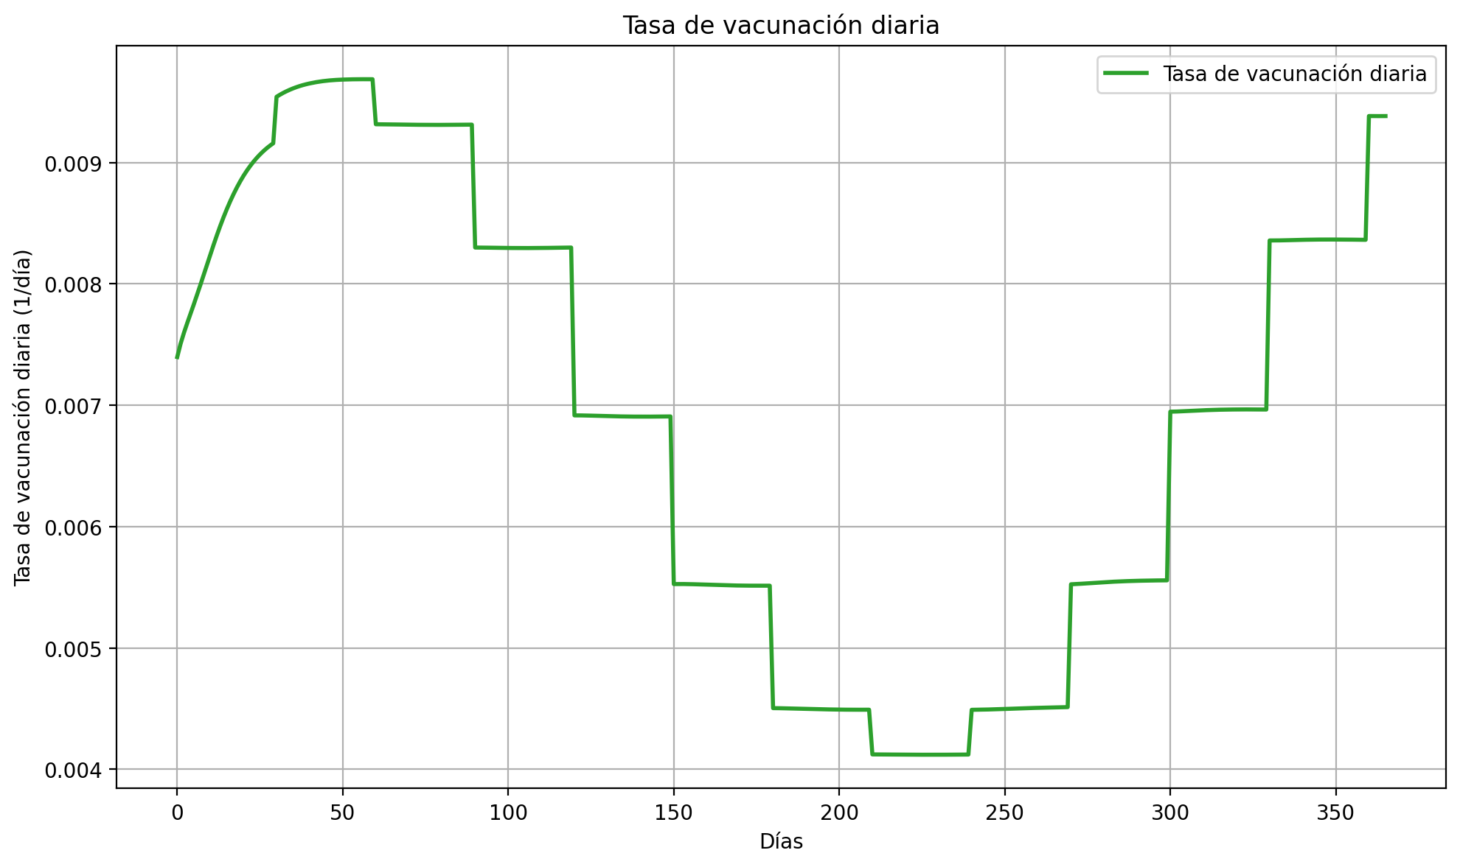
\includegraphics[width=0.85\textwidth]{Images/tasa_vacc.png}
\captionof{figure}{Tasa diaria de vacunación a lo largo del tiempo (solo escenario con vacunación).}


La Figura muestra la evolución de la tasa de vacunación diaria $\nu(t)$ a lo largo del año. 

\paragraph{Inicio elevado de la tasa vacunal.} La curva comienza con un crecimiento rápido de la tasa vacunal desde el inicio del año hasta aproximadamente el día 60, alcanzando valores cercanos a 0.0095. Esto es coherente con el aumento inicial de infectados observado en las curvas de $I_h$ y $E_h$, y con la estacionalidad de la transmisión, que presenta su punto álgido en febrero.

\paragraph{Reducción progresiva (días 60–180).} A medida que la epidemia se controla parcialmente, la tasa de vacunación disminuye gradualmente. Esto sugiere una menor presión epidemiológica y refleja la acción del modelo adaptativo: la necesidad de vacunación decrece cuando los niveles de infección disminuyen.

\paragraph{Mínimo vacunal (días 180–260).} En el tercer trimestre del año, la tasa alcanza su punto más bajo (~0.004), coincidiendo con el momento de menor incidencia en los compartimentos $I_h$ y $E_h$. Este comportamiento también puede relacionarse con una menor percepción de riesgo, como ocurre en campañas reales donde el descenso de casos puede llevar a una relajación en las estrategias preventivas.

\paragraph{Reactivación vacunal (días 270–365).} En el último tercio del año, la curva muestra un ascenso progresivo de $\nu(t)$, en respuesta al rebrote epidémico evidenciado en las curvas de $I_h$, $E_h$ y $S_h$. El modelo reactivo permite ajustar automáticamente el esfuerzo vacunal ante esta nueva ola de transmisión, anticipando el nuevo pico estacional.

\paragraph{Conclusión.} La estrategia vacunal utilizada, basada en la modulación de la tasa diaria $\nu(t)$, permite una asignación inteligente y oportuna de recursos. Su comportamiento se alinea de forma lógica con la dinámica epidemiológica y estacional de la leptospirosis, maximizando la eficiencia del control y minimizando vacunaciones innecesarias fuera de los periodos críticos.



\subsubsection[Análisis de la Dinámica de Vectores (Sv, Iv, Rv)]{Análisis de la Dinámica de Vectores (\texorpdfstring{$S_v$, $I_v$, $R_v$}{Sv, Iv, Rv})}

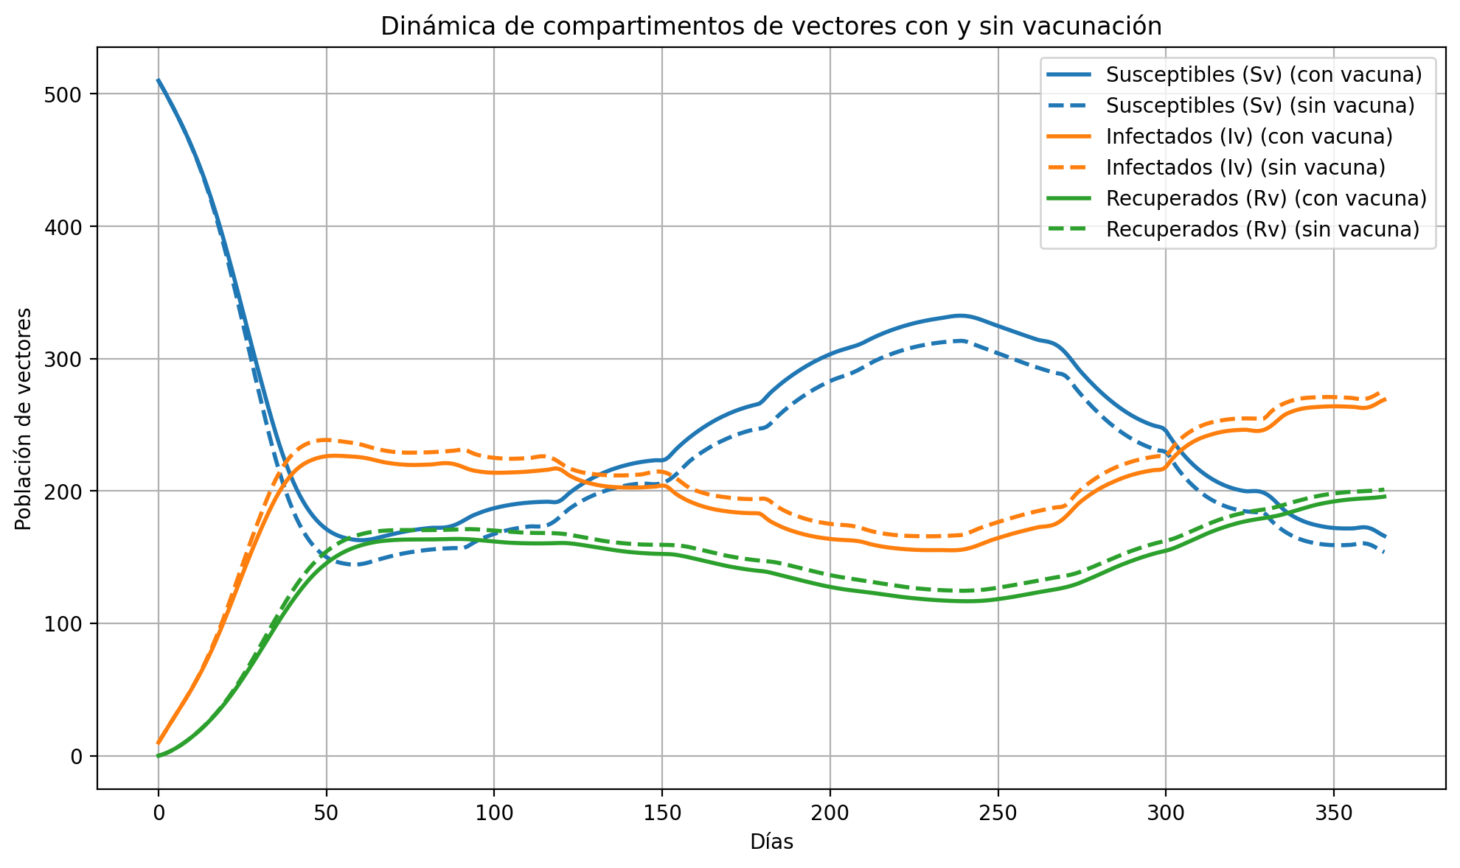
\includegraphics[width=0.85\textwidth]{Images/vectores.png}
\captionof{figure}{Dinámica anual de la población de roedores: susceptibles ($S_v$), infectados ($I_v$) y recuperados ($R_v$) bajo escenarios con y sin vacunación humana.}

La Figura presenta la evolución anual de los compartimentos de la población de vectores (roedores) susceptibles ($S_v$), infectados ($I_v$) y recuperados ($R_v$), tanto en escenarios con vacunación humana como sin ella. Aunque los roedores no son vacunados, su dinámica se ve influenciada indirectamente por la reducción de la carga infecciosa humana, dado que el modelo considera transmisión inversa humano-vector.

\paragraph{Susceptibles ($S_v$).} En ambos escenarios, la población susceptible de roedores decrece rápidamente durante las primeras semanas, debido al aumento de infecciones transmitidas desde humanos infectados ($I_h$) y el ambiente contaminado ($B_l$). Sin embargo, el escenario con vacunación muestra una recuperación progresiva más marcada de $S_v$, especialmente entre los días 100 y 300. Esto sugiere que la reducción de $I_h$ mediante vacunación contribuye a una menor presión de transmisión sobre la población roedora.

\paragraph{Infectados ($I_v$).} La población de roedores infectados alcanza su punto máximo cerca del día 50 en ambos escenarios, con valores ligeramente mayores sin vacunación. A partir de ese punto, la curva en el escenario con vacunación se mantiene sistemáticamente por debajo, indicando que la transmisión humano-vector se ve mitigada indirectamente por el control en humanos. Esta observación es coherente con lo reportado en modelos ecoepidemiológicos con retroalimentación entre hospedadores y vectores \cite{kassa2021}.

\paragraph{Recuperados ($R_v$).} Ambas curvas de recuperados roedores muestran una acumulación gradual, siendo ligeramente más baja con vacunación humana. Esto es congruente con la menor exposición general del vector al patógeno en ese escenario, que da lugar a menos conversiones $I_v \rightarrow R_v$. A pesar de ello, las curvas convergen hacia finales del año, lo que sugiere una estabilización del ecosistema infeccioso.

\paragraph{Implicancias epidemiológicas.} Aunque la intervención se aplica exclusivamente sobre la población humana, sus efectos se transmiten a la dinámica del vector. Reduciendo la carga humana ($I_h$), se disminuye también la probabilidad de que un roedor se infecte al contacto con ambientes contaminados o fluidos humanos, lo que termina afectando positivamente al sistema entero.

\paragraph{Conclusión.} La vacunación humana no sólo protege a las personas directamente, sino que también genera externalidades positivas sobre la población vectorial, disminuyendo la presión infecciosa a través de la transmisión inversa. Esto refuerza la necesidad de abordar las zoonosis desde un enfoque de salud única o One Health, como recomienda la OMS y la FAO.


\subsubsection[Análisis de la Dinámica de Bacterias en el Ambiente (Bl)]{Análisis de la Dinámica de Bacterias en el Ambiente ($B_l$)}


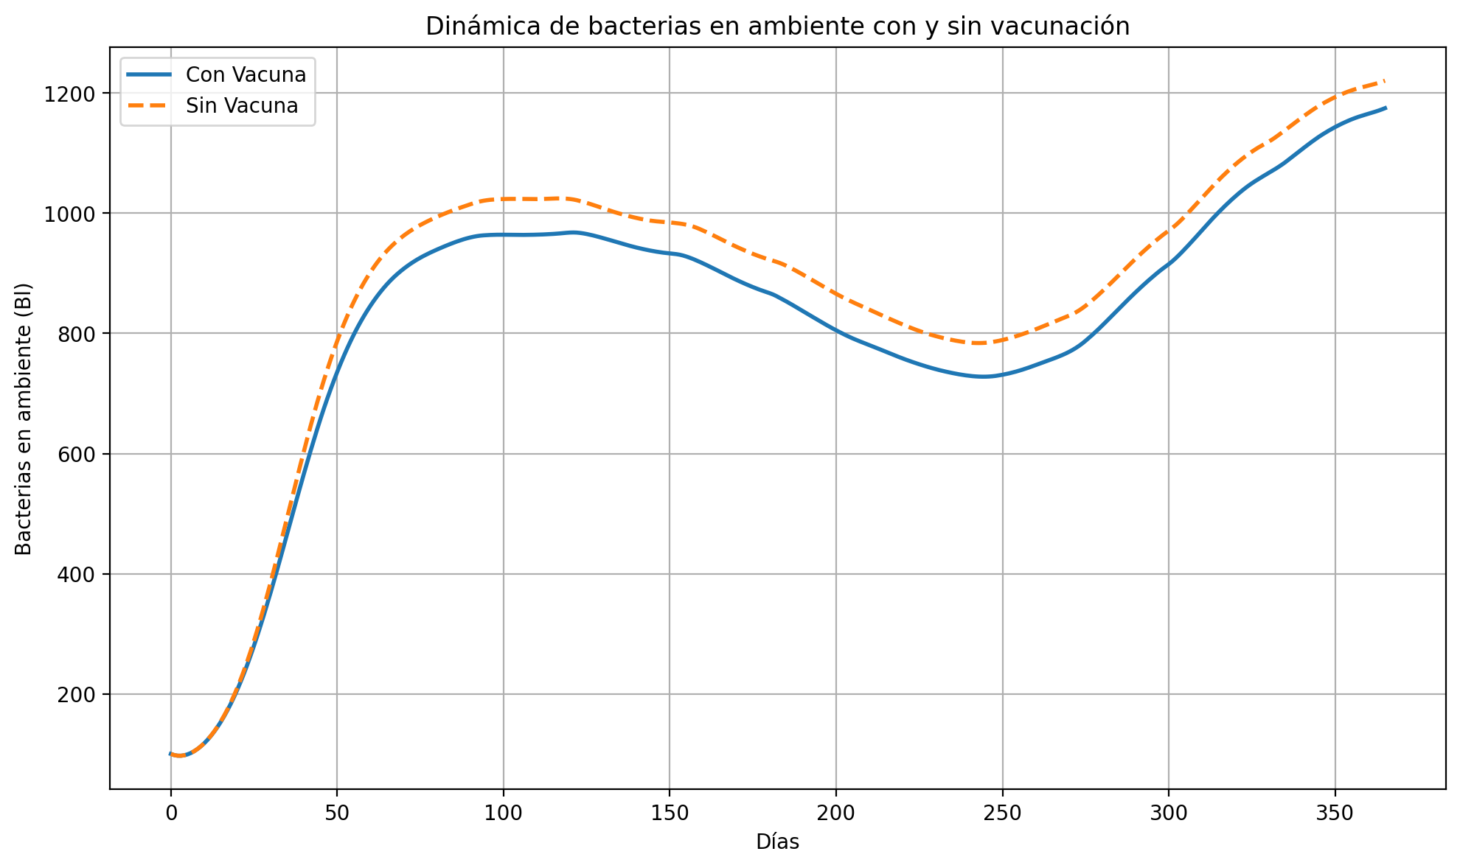
\includegraphics[width=0.85\textwidth]{Images/ambiente.png}
\captionof{figure}{Dinámica de bacterias ambientales: comparación entre escenarios sin y con vacunación.}

La Figura muestra la evolución temporal del compartimento $B_l$, que representa la cantidad de bacterias \textit{Leptospira} presentes en el ambiente (agua, suelo, zonas húmedas) en los escenarios con y sin vacunación humana. Este compartimento es esencial en la modelación ecoepidemiológica de la leptospirosis, pues actúa como reservorio infeccioso y amplificador de la transmisión indirecta.


\paragraph{Ascenso inicial (días 0–60).} Ambas curvas muestran un crecimiento rápido en la carga ambiental de bacterias, alcanzando un primer máximo cercano al día 60. Esto está asociado al aumento de individuos infectados ($I_h$ e $I_v$), quienes excretan leptospiras al ambiente. La curva sin vacunación alcanza valores ligeramente más altos debido a la mayor prevalencia de infección en humanos y roedores, como se evidenció en los gráficos anteriores.

\paragraph{Meseta y descenso (días 60–200).} Posteriormente, ambas curvas entran en una fase de meseta y descenso, con una diferencia constante a favor del escenario vacunado. La reducción en $I_h$ e $I_v$ debido a la vacunación disminuye el flujo bacteriano hacia el ambiente. Este fenómeno coincide con estudios que muestran que el control de los reservorios infecciosos humanos y animales reduce sustancialmente la contaminación ambiental \cite{trueba2019}.

\paragraph{Rebrote ambiental (días 250–365).} En el último tercio del año se observa un nuevo ascenso de $B_l$, coincidiendo con el segundo pico epidémico en los compartimentos de humanos infectados. Sin embargo, la curva con vacunación mantiene una trayectoria inferior, lo que sugiere que la estrategia vacunal también modera la carga ambiental al reducir la incidencia clínica.

\paragraph{Persistencia y riesgo.} Cabe destacar que la diferencia entre ambas curvas, aunque presente, no es tan marcada como en otros compartimentos. Esto se debe a la alta capacidad de \textit{Leptospira} para sobrevivir en ambientes húmedos durante semanas o meses, dependiendo de factores como temperatura, pH y radiación UV. Esto sugiere que, si bien la vacunación reduce la contaminación ambiental, no la elimina, y debe ser complementada con medidas de saneamiento e intervención ambiental.

\paragraph{Conclusión.} El modelo confirma que la vacunación humana tiene un efecto indirecto y positivo en la reducción de la carga bacteriana ambiental, contribuyendo a cortar el ciclo ecoepidemiológico de la leptospirosis. Sin embargo, la persistencia del patógeno en el ambiente justifica acciones adicionales de control ecológico y mejoras en la infraestructura sanitaria.


\newpage
% ================================
\section{Análisis Costo-Beneficio}

\subsection{Metodología y parámetros utilizados}

El análisis de costo-beneficio realizado considera los siguientes elementos:

\begin{itemize}
    \item \textbf{Casos evitados:} Se calcula la diferencia entre la incidencia acumulada de infecciones humanas en los escenarios sin vacunación y con vacunación. La incidencia acumulada se estima integrando  el número de nuevos infectados ($\theta E_h$) a lo largo del periodo simulado.
    \item \textbf{Costos de vacunación:} Se calcula como el producto del número total de personas vacunadas (integral de la tasa diaria de vacunación sobre los susceptibles), el costo por dosis y el número de dosis requeridas por persona.
    \item \textbf{Ahorros sanitarios:} Se estima multiplicando el número de casos evitados por la proporción de casos leves, moderados y graves, y el costo promedio asociado a cada tipo de caso.
    \item \textbf{Beneficio neto:} Diferencia entre los ahorros sanitarios y el costo total de la vacunación.
    \item \textbf{Ratio beneficio/costo:} Cociente entre los ahorros sanitarios y el costo de vacunación, indicador clave de rentabilidad.
\end{itemize}


\subsection{Costos asociados a la leptospirosis en Brasil y la vacuna Vax-SPIRAL®}

\begin{itemize}
    \item \textbf{Costo por dosis de Vax-SPIRAL®:} USD 15. Este valor es una estimación asumida para el análisis, ante la ausencia de información pública sobre el precio comercial de la vacuna. La cifra se basa en rangos típicos de vacunas bacterianas en América Latina y puede variar según acuerdos institucionales y subsidios.

    \item \textbf{Proporción de casos leves:} 85\% (estimado global, incluye formas subclínicas y sintomáticas leves) \cite{who2022}.  

    \item \textbf{Proporción de casos moderados:} 5\%

    \item \textbf{Proporción de casos graves:} 10\% (requieren hospitalización, con letalidad del 5-30\%) \cite{who2022,msbrasil2021}.  

    \item \textbf{Costo caso leve:} $\sim$USD 159 (R\$ 795,60\footnotemark[1]). Incluye diagnóstico ambulatorio (serología, PCR), antibioticoterapia (doxiciclina/amoxicilina) y seguimiento \cite{who2022,souza2011}.  

    \item \textbf{Costo caso moderado:} $\sim$USD 1,996 (R\$ 9,980\footnotemark[1]). Hospitalización media de 6 días, medicamentos intravenosos y soporte renal \cite{souza2011}.  

    \item \textbf{Costo caso grave:} $\sim$USD 33,260 (R\$ 166,300\footnotemark[1]). Incluye UCI, diálisis, transfusión y complicaciones (síndrome de Weil). Costo parcial de hospitalización en Brasil (2007) fue R\$831,500 para múltiples casos \cite{souza2011}.  
\end{itemize}

\footnotetext[1]{Conversión: R\$ 5,00 = USD 1,00 (tasa promedio 2025). Costos originales en reales (R\$) del estudio de Souza et al. (2011) \cite{souza2011}.}




\subsection{Resultados}
\begin{table}[H]
\centering
\begin{tabular}{@{}ll@{}}
\toprule
\textbf{Indicador} & \textbf{Valor} \\
\midrule
Infecciones evitadas & 497 \\
Ahorro sanitario total & \$1,770,414.76 \\
Costo de vacunación & \$5,975.61 \\
Beneficio neto & \$1,764,439.16 \\
Ratio beneficio/costo & 296.27 \\
\bottomrule
\end{tabular}
\caption{Resultados del análisis de costo-beneficio para la vacunación contra leptospirosis.}
\end{table}

Los resultados muestran que la estrategia de vacunación permitiría evitar 497 infecciones humanas en un año, generando un ahorro sanitario estimado en \$1,770,414.76. El costo directo de la vacunación sería de \$5,975.61, lo que resulta en un beneficio neto de \$1,764,439.16 y un ratio beneficio/costo de 296.27. Esto significa que, por cada dólar invertido en vacunación, se ahorran aproximadamente 296 dólares en costos sanitarios asociados a la enfermedad, lo que confirma que la intervención es altamente costo-efectiva.

Cabe destacar que este análisis considera únicamente el costo de las dosis de vacuna y no incluye otros gastos operativos de la campaña, como personal, logística o infraestructura. Aun así, la magnitud del ahorro sanitario sugiere que la vacunación seguiría siendo económicamente favorable incluso contemplando estos costos adicionales.

\newpage

% ================================
\section{Análisis de Sensibilidad}

\newpage
% ================================
\section{Conclusiones}

El modelo matemático desarrollado demuestra la utilidad de incluir estrategias de vacunación para reducir la carga de leptospirosis. Las simulaciones muestran claras ventajas en términos de reducción de infectados y rentabilidad económica. Además, el análisis de sensibilidad respalda la importancia de lograr coberturas elevadas.

% ================================
\section{Limitaciones}

\begin{itemize}
\item Supuestos como homogeneidad poblacional y parámetros constantes limitan la precisión del modelo.
\item La estimación de costos es preliminar y puede variar según el contexto.
\end{itemize}

\newpage
% ================================
\section{Próximos pasos}

\begin{itemize}
\item Incorporar datos reales para validación.
\item Explorar distintos esquemas de vacunación estacionales o focalizados.
\item Ampliar el modelo con intervención vectorial y factores ambientales.
\end{itemize}

% ================================

% ================================
\section{Anexos}

\subsection{Software desarrollado}

Como parte de este trabajo, se desarrolló una herramienta interactiva en Python utilizando \texttt{streamlit} para la simulación y visualización del modelo SEIR extendido con vacunación. El software permite al usuario modificar parámetros, explorar distintos escenarios y visualizar los resultados de manera gráfica e intuitiva.

El código fuente y la documentación están disponibles en el repositorio de GitHub:

\begin{center}
\url{https://github.com/Pol4720/vax-SPIRAL-CB}
\end{center}

\textbf{Características principales:}
\begin{itemize}
    \item Interfaz web interactiva usando \texttt{streamlit}.
    \item Simulación de escenarios con y sin vacunación.
    \item Ajuste de parámetros epidemiológicos y de vacunación.
    \item Visualización de la dinámica de todos los compartimentos del modelo.
    \item Análisis de sensibilidad y exportación de resultados.
\end{itemize}

\textbf{Requisitos:}
\begin{itemize}
    \item Python 3.8 o superior.
    \item Paquetes: \texttt{streamlit}, \texttt{numpy}, \texttt{scipy}, \texttt{matplotlib}, \texttt{pandas}.
\end{itemize}

\textbf{Ejecución local:}
\begin{verbatim}
git clone https://github.com/Pol4720/vax-SPIRAL-CB.git
cd vax-SPIRAL-CB
cd Tools
pip install -r requirements.txt
streamlit run app.py
\end{verbatim}

Para más detalles y ejemplos de uso, consulte el archivo \texttt{README.md} en el repositorio.
\section{Bibliografía}
\begin{thebibliography}{9}

\bibitem{who2022} 
Organización Mundial de la Salud. (2022). Leptospirosis: epidemiología y carga de enfermedad. Informe técnico.

\bibitem{msbrasil2021} 
Ministerio de Salud de Brasil. (2021). Guía de vigilancia epidemiológica: leptospirosis.

\bibitem{souza2011} 
Souza, V. et al. (2011). Costos hospitalarios de la leptospirosis en Brasil. \textit{Revista de Saúde Pública}, 45(6), 1124-1133.

\bibitem{who} Organización Mundial de la Salud. Leptospirosis. Disponible en: \url{https://www.who.int/news-room/fact-sheets/detail/leptospirosis}


\bibitem{engida2022}
Engida, H. A., Theuri, D. M., Gathungu, D., Gachohi, J., \& Alemneh, H. T. (2022).
A Mathematical Model Analysis for the Transmission Dynamics of Leptospirosis Disease in Human and Rodent Populations.
\textit{Computational and Mathematical Methods in Medicine}, 2022, Article ID 1806585.

\bibitem{paisanwarakiat2021}
Paisanwarakiat, R. and Thamchai, R. (2021).
Optimal Control of a Leptospirosis Epidemic Model.
\textit{Science \& Technology Asia}, 2021.

\bibitem{minter2019}
Minter, A., Costa, F., Khalil, H., et al. (2019).
Optimal control of rat-borne leptospirosis in an urban environment.
\textit{Frontiers in Ecology and Evolution}, 7, 209.

\bibitem{alemneh2020}
Alemneh, H. T. (2020).
A co-infection model of dengue and leptospirosis diseases.
\textit{Advances in Difference Equations}, 2020, 23 pages.

\bibitem{khan2012}
M. A. Khan, G. Zaman, S. Islam, and M. I. Chohan,
``Optimal campaign in leptospirosis epidemic by multiple control variables,''
\textit{Applied Mathematics}, vol. 3, no. 11, pp. 1655--1663, 2012.

\bibitem{khan2014}
M. A. Khan, S. Islam, S. A. Khan, I. Khan, S. Shafie, and T. Gul,
``Prevention of leptospirosis infected vector and human population by multiple control variables,''
\textit{Abstract and Applied Analysis}, vol. 2014, Article ID 619035, 9 pages, 2014.


\bibitem{pijnacker2019}
Pijnacker, R., Goris, M. G. A., Wagenaar, J. F. P., Hartskeerl, R. A., Lauwerends, L. J., van der Hoek, W., \& Schimmer, B. (2019).
Evaluating Leptospirosis Burden and Risk in the Netherlands Through Spatial Modelling and Surveillance Data.
\textit{PLoS Neglected Tropical Diseases}, 13(9), e0007780.

\bibitem{cdc2024}
Centers for Disease Control and Prevention.
Leptospirosis - CDC Fact Sheet.
2024.
\url{https://www.cdc.gov/leptospirosis/index.html}

\bibitem{adler2010}
Adler, B., \& de la Peña Moctezuma, A. (2010).
Leptospira and leptospirosis.
\textit{Veterinary Microbiology}, 140(3-4), 287--296.

\bibitem{goris2020}
Goris, M. G. A., \& Hartskeerl, R. A. (2020).
Duration of immunity following vaccination against leptospirosis: A review of the available evidence.
\textit{Vaccine}, 38(52), 8326--8335.

\bibitem{who2023}
World Health Organization.
Operational framework for managing zoonotic disease epidemics using One Health: WHO guidance.
2023.
\url{https://www.who.int/publications/i/item/9789240074441}

\bibitem{kassa2021}
Kassa, S. M., et al. (2021).
Impact of host vaccination on vector-borne disease dynamics in a zoonotic context.
\textit{Ecological Modelling}, 455, 109643.

\bibitem{trueba2019}
Trueba, G., Zapata, S., Madrid, K., \& Cullen, P. (2019).
Survival of pathogenic leptospira in the environment and its implications for leptospirosis control.
\textit{Revista Panamericana de Salud Pública}, 43, e61. PAHO.


\end{thebibliography}

\end{document}